\section{Preliminaries and notation}

We recall here some additional terminology on $\HH$. We have $\mathfrak{h}:=\mathrm{Lie}(\HH)=\mathrm{span}\{X,Y\}\oplus\mathrm{span}\{Z\}$ with the only nontrivial bracket relation being $[X,Y]=Z$. Let us recall that the \textit{Kor\'anyi norm} of $(x,y,z)\in\HH$ is:
\begin{equation}\label{eq:def-koranyi}
  |(x,y,z)|_K:=\sqrt[4]{(x^2+y^2)^2+16 z^2},
\end{equation}
and that we denote by
\begin{equation}\label{eq:koranyi}
d(a,b):=|b^{-1}\cdot a|_K,
\end{equation}
the \textit{Kor\'anyi distance}. The distance $d$ is bi-Lipschitz equivalent to any Carnot--Carathéodory distance on $\HH$. If $a=(x_a,y_a,z_a)$ and $b=(x_b,y_b,z_b)$, then 
\begin{equation}\label{eqn:dab}
    d(a,b)^2=\sqrt{((x_a-x_b)^2+(y_a-y_b)^2)^2+16z(b^{-1}\cdot a)^2},
\end{equation}
where $z(b^{-1}\cdot a)$ is the $z$--coordinate of $b^{-1}\cdot a$, i.e., 
\[
z(b^{-1}\cdot a)=z_a-z_b+\frac{1}{2}\left(x_a y_b-x_b y_a\right).
\]

\section{Geometry and topology of vertical curves}\label{sec:Properties}
In this section, we prove some properties of vertical curves, including Proposition~\ref{prop:Properties}.Unlike intrinsic Lipschitz graphs, vertical curves cannot be naturally viewed as graphs over a subgroup of $\HH$. Indeed, if $\gamma\from I\to \HH$ is a vertical map, there need not be a $p$ such that $p\cdot\gamma(t)$ has nondecreasing $z$--coordinate. 

Nonetheless, we will show that connected vertical curves are homeomorphic to intervals and that the homeomorphism can be taken to be bi-H\"older on compact sets.

We will need the following relation on $\HH$. For $p,q\in \HH$,
\begin{equation}\label{eq:def-order}
  p\prec q \qquad \text{if and only if } z(p^{-1}q)>0.
\end{equation}
Note that $z(p^{-1}q) = -z(q^{-1}p)$, so $p\prec q$ and $q \prec p$ are mutually exclusive. This is not a partial order on $\HH$ because it is nontransitive; one can show that $X \prec Y^{-1} \prec X^{-1} \prec Y \prec X$. Regardless, we will show that it induces a total order on connected vertical curves and use this to describe the geometry and topology of connected vertical curves.

The main results of this section are the following lemma and proposition.
\begin{lemma}\label{lem:Properties}
 Let $\lambda>0$, and let $E\subset \HH$ be a $\lambda$--vertical curve. Then:
  \begin{enumerate}
  \item For every $p\in\HH$, $p\cdot E$ is a $\lambda$--vertical curve.
  \item For every $\rho>0$, $s_\rho(E)$ is a $\lambda$--vertical curve.
  \item\label{Item3} If $\lambda > \frac{1}{4}$, or if $E$ is connected, then \eqref{eq:def-order} defines a total order on $E$. Moreover, if $E$ is the image of an injective map $\gamma\from I\to\HH$, then $\gamma$ is either monotone increasing in the sense that
  \begin{equation}\label{eqn:First}
  \gamma(s) \prec \gamma(t) \quad \forall s<t,
  \end{equation}
  or it is monotone decreasing in the sense that
  \begin{equation}\label{eqn:Second}
  \gamma(s) \succ \gamma(t) \quad \forall s<t.
  \end{equation}
  \item\label{Item4} 
    There is a $c_\lambda>0$ such that for all $a,b,c\in E$ such that $a\prec b$, $b\prec c$, and $a\prec c$,
    \begin{equation}\label{eq:coarse-monotone}
      z(a^{-1}\cdot c)\geq c_\lambda z(a^{-1}\cdot b) \text{ and } d(a,c)\geq c_\lambda d(a,b).
    \end{equation}
\end{enumerate}
\end{lemma}

\begin{prop}\label{prop:intervals}
  Let $\lambda>0$ and let $E$ be a connected $\lambda$--vertical curve. Then $E$ is homeomorphic to an interval and thus $E$ is parametrized by an increasing $\lambda$--vertical map $\gamma\from I \to\HH$.
\end{prop}
In fact, $E$ is locally bi-H\"older equivalent to an interval; see Lemma~\ref{lem:biHolderonCompact}.

We will first prove Lemma~\ref{lem:Properties}. Let
$$
\VCone_\lambda^+:=\VCone_\lambda\cap\{z\geq 0\}, \quad \VCone_\lambda^-:=\VCone_\lambda\cap\{z\leq 0\}.
$$ 

\begin{proof}[Proof of Lemma~\ref{lem:Properties}]
    Parts (1) and (2) are a direct consequence of the definitions, and the fact that $\VCone_\lambda$ is $s_\rho$-invariant.

Let us now prove part (3). Note that for every $p, q\in E$, we have $q\in \VCone_\lambda^+\cup\VCone_\lambda^-$, so $p\preceq q$ or $q\preceq p$. 
In order to prove part (3), we need to prove that the relation \eqref{eq:def-order} is transitive on $E$.

We first consider the case that $\lambda>\frac{1}{4}$. Let $a, b, c\in E$ and suppose $a\prec b$ and $b\prec c$. Then $g = a^{-1} b\in \VCone_\lambda^+$ and $h = b^{-1} c\in \VCone_\lambda^+$, i.e., $z(g) > \frac{1}{4}|\pi(g)|^2$ and $z(h) > \frac{1}{4}|\pi(h)|^2$. We claim that $a\prec c$, i.e., that $z(a^{-1}c) = z(gh) > 0$.

We have
\[
\begin{aligned}
z(gh) &= z(g) + z(h) + \frac{1}{2}\big(x(g) y(h) - x(h) y(g)\big) \\ &\ge z(g) + z(h) - \frac{1}{2}|\pi(g)||\pi(h)|,
\end{aligned}
\]
and
$$
\frac{1}{2}|\pi(g)||\pi(h)|<2\sqrt{z(g)z(h)}\le z(g)+z(h),
$$
by the arithmetic-geometric mean inequality. Therefore,
$$
z(gh) \ge z(g) + z(h) - \frac{1}{2}|\pi(g)||\pi(h)| > 0,
$$
which implies $a\prec c$.

Next, suppose that $E$ is connected. We again let $a, b, c\in E$ such that $a\prec b$ and $b\prec c$.
For $p\in E$, let 
\[
E_p^+:=\{x\in E : x\succ p\}, \quad E_p^-:=\{x\in E : x\prec p\}.
\]
Then $E\setminus\{p\}=E_p^+\sqcup E_p^-$, i.e., $E_p^+,E_p^-$ are disjoint, relatively open sets that cover $E\setminus\{p\}$. It follows that any connected component of $E\setminus\{p\}$ lies in one or the other. In particular, $a$ and $c$ are in different connected components of $E\setminus \{b\}$. 

Let $A$ be the connected component of $a$ in $E\setminus\{b\}$. Since $E$ is connected, the closure $\overline{A}$ of $A$ in $E$ contains $b$; since $a$ and $c$ are in different connected components of $E\setminus \{b\}$, $c\not \in \overline{A}$. Therefore, $\overline{A}$ is a connected subset of $E\setminus\{c\}$ that contains $a$ and $b$. Since $b\prec c$, this implies $a\prec c$, as desired.

Finally, let $\gamma\from I\to \HH$ be a $\lambda$--vertical map. Let $f\from I^2 \to \R$,  $f(s,t)=z(\gamma(s)^{-1}\gamma(t))$. Then $f(s,t)\ne 0$ for all $(s,t)$ such that $s\ne t$. In particular, either $f(s,t)>0$ for all $s<t$ or $f(s,t)<0$ for all $s<t$. In the first case, $\gamma(s)\prec \gamma(t)$ for all $s<t$; in the second case, $\gamma(s)\succ \gamma(t)$ for all $s<t$.

We now consider part (4). After a left-translation we may suppose that $a=\0$. Let $b=(x_b,y_b,z_b)$, and $c = (x_c,y_c,z_c)$. Then on one hand, since $c\succ b$, 
$$0\le z(b^{-1}c) = -z_b + z_c + \frac{1}{2}(-x_by_c+x_cy_b) \le -z_b + z_c + \frac{1}{2} |\pi(b)||\pi(c)|,$$
i.e.,  
\begin{equation}\label{eq-zc-lower-1}
  z_c \ge z_b - \frac{1}{2} |\pi(b)||\pi(c)|.
\end{equation}
Since $b\succ \0$, we have $|\pi(b)|\le \sqrt{z_b \lambda^{-1}}$. Thus, on one hand, if 
$|\pi(c)| \le \sqrt{z_b \lambda}$, then 
$$z_c \ge z_b - \frac{1}{2} \sqrt{z_b \lambda^{-1}}\sqrt{z_b \lambda} \ge \frac{z_b}{2}.$$
On the other hand, if $|\pi(c)| \ge \sqrt{z_b \lambda}$, then since $c\succ \0$, we have
$$z_c \ge \lambda(\sqrt{z_b \lambda})^2 = \lambda^2 z_b.$$
In either case, $z_c\ge \min\{\frac{1}{2},\lambda^2\} z_b$. 

Since $E$ is $\lambda$--vertical, if $p,q\in E$, then $d(p,q)\approx_\lambda |z(p^{-1}q)|$, i.e., $z_b\approx_\lambda d(a,b)$ and $z_c\approx_\lambda d(a,c)$. Therefore, there is a $c_\lambda>0$ such that $d(a,c)\ge c_\lambda d(a,b)$, as desired.
\end{proof}

The proof of  Proposition~\ref{prop:intervals} uses the following two lemmas.
\begin{lemma}\label{lem:compact-intersections}
  Let $\lambda>0$. There is a $C>0$ such that for all $p,q\in \HH$, if $q\in p\VCone_\lambda^+$, then
  $$\diam\left(p\VCone_\lambda^+\cap q \VCone_\lambda^-\right)\le C d(p,q).$$
  In particular, if $E$ is a $\lambda$--vertical curve and $p,v,q\in E$ are such that $p\prec v$, $v\prec q$, and $p\prec q$, then $d(p,v)\le C d(p,q)$.
\end{lemma}
\begin{proof}
  It suffices to prove the lemma when $p=\0$.
  Let $c_\lambda$ be as in Lemma~\ref{lem:Properties}.(\ref{Item4}), let $D=\VCone_\lambda^+\cap q \VCone_\lambda^-$, and let $v\in D$. Then $\0 \prec v$, $v\prec q$, and $\0 \prec q$, so by \eqref{eq:coarse-monotone}, $z(q) \ge c_\lambda z(v)$. By \eqref{eq:def-koranyi},
  $$
  z(v) \le c_\lambda^{-1} z(q) \le \frac{c_\lambda^{-1} d(\0,q)^2}{4}.
  $$
  Furthermore, since $v\in \VCone_\lambda^+$,
  $$
  |\pi(v)| \le \sqrt{z(v)\lambda^{-1}} \le d(\0,q) \sqrt{\frac{c_\lambda^{-1}\lambda^{-1}}{4}}.
  $$
  Therefore, if $C=\sqrt{c_\lambda^{-1}\lambda^{-1}/4} + \sqrt{c_\lambda^{-1}}$, then
  $$
  d(\0,v) = \sqrt[4]{|\pi(v)|^4+16 z(v)^2} \le C d(\0,q),
  $$
  as desired. 
\end{proof}

\begin{lemma}\label{lem:topologies}
  Let $\lambda>0$. Suppose that $E\subset \HH$ is a closed $\lambda$--vertical curve which is totally ordered, i.e., if $p,q,r\in E$, $p\prec q$, and $q\prec r$, then $p\prec r$. Then the
  order on $E$ is complete and the
  subset topology on $E$ coincides with the order topology, i.e., the topology generated by the rays
$I_{a,\infty}:=\{z\in E:a\prec z\}$ and $I_{-\infty,a}:=\{z\in E:z\prec a\}$, and the intervals $I_{a,b}:=\{z\in E:a\prec z\prec b\}$, with $a,b\in E$.
\end{lemma}
\begin{proof}
  (Unless we specify the order topology, topological notions in this proof will refer to the subset topology on $E$.)
  
  We first show that the order is complete, i.e., that every non-empty subset of $E$ with an upper bound has a least upper bound and every non-empty subset of $E$ with a lower bound has a greatest upper bound.

  Let $S$ be a subset of $E$ that is bounded above by some $M$; the case that $S$ is bounded below is similar. Let $\{a_1,\ldots,a_n,\ldots\}\subset S$ be a countable dense subset. For $i\ge 1$, let  $m_i=\max\{a_1,\ldots,a_i\}$. Then 
  $$
  m_i\in m_1\VCone_\lambda^+\cap M\VCone_\lambda^-, \quad \forall i\geq 0.
  $$ 
  By Lemma~\ref{lem:compact-intersections}, this intersection is compact, so there is a subsequence of $m_i$ that converges to some $v\in \HH$. Since $E$ is closed, $v\in E$, and one can check that $v$ is the least upper bound of $S$. Thus the order on $E$ is complete.

  Note that this argument also proves that if $S\subset E$ is bounded above, then $\sup S$ is a limit point of $S$ in the subset topology. 

  Now, we compare the order topology and the subset topology. For every $a,b\in E$ with $a\prec b$,
  $$I_{a,b} = E \cap \left(\HH \setminus (a \VCone_\lambda^- \cup b \VCone_\lambda^+)\right),$$
  so $I_{a,b}$ is open in the subspace topology (as are $I_{-\infty,a}$ and $I_{a,\infty}$). That is, the subspace topology is finer than the order topology.

  Conversely, let $p\in E$ and $\delta>0$. 
  We will show that there is an open set $U\subset E$ in the order topology such that $p \in U \subset B_\delta(p)$. 

  First, we claim that there is some $t\in I_{p,\infty} \cup \{\infty\}$ such that $I_{p,t}\subset B_\delta(p)$. Suppose that $I_{p,\infty}$ is nonempty; otherwise, we take $t=\infty$ and check that $I_{p,t} =\emptyset \subset B_\delta(p)$. By completeness, $I_{p,\infty}$ has a greatest lower bound $q$. If $q\ne p$, then $I_{p,q}=\emptyset$, so we suppose that $p=q$. By the above, $p$ is a limit point of $I_{p,\infty}$ in the subspace topology, i.e., for every $r>0$, the set $B_r(p)\cap I_{p,\infty}$ is nonempty.

  Let $C$ be as in Lemma~\ref{lem:compact-intersections} and let $t\in B_{C^{-1}\delta}(p)\cap I_{p,\infty}$. For all $v\in I_{p,t}$, we have $p\prec v\prec t$, so by Lemma~\ref{lem:compact-intersections}, $I_{p,t} \subset B_\delta(p)$, as desired.

  Likewise, there is some $s\in \{-\infty\} \cup I_{-\infty,p}$ such that $I_{s,p}\subset B_\delta(p)$. Then $s\prec p\prec t$, and
  $$I_{s,t} = I_{s,p}\cup \{p\}\cup I_{p,t}\subset B_\delta(\0).$$
  Thus the order topology is finer than the subspace topology, so the two topologies coincide.  
\end{proof}

We will use these lemmas to prove Proposition~\ref{prop:intervals}. 

\begin{proof}[Proof of Proposition~\ref{prop:intervals}]
  Let $E\subset \HH$ be a connected $\lambda$--vertical subset. We claim that $E$ is homeomorphic to an interval.
If we prove the assertion when $E$ is closed, then we are done. Indeed, if $E$ is not closed, then $E\subset\overline{E}$ is homeomorphic to a connected subset of an interval, and thus $E$ itself is homeomorphic to an interval, as desired.

Hence, we assume $E$ is closed. Since $E$ is connected, Lemma~\ref{lem:Properties}.(\ref{Item3}) implies that $E$ is totally ordered. Thus, by Lemma~\ref{lem:topologies}, the order on $E$ is complete and the order topology on $E$ agrees with the subset topology.

We claim that the order on $E$ is separable and dense. Since $E$ is separable in the subset topology, it is separable in the order topology. The density of the order follows from the connectedness of $E$. That is, if $p,q\in E$ and $p\prec q$, then $I_{p,q}$ is nonempty; otherwise $I_{-\infty,q}$ and $I_{p,\infty}$ would be disjoint open subsets of $E$ that cover $E$. 

The conclusion then follows from a classical result due to Cantor on complete, separable, dense orders. Let $E'$ be $E$ without its endpoints, if any, and let $\mathcal{D}$ be a countable dense subset of $E'$. By a theorem of Cantor, any such subset is order-isomorphic to $\mathbb Q\cap (0,1)$. The completeness of $E$ lets us extend this isomorphism to an isomorphism from $E'$ to the interval $(0,1)$. This isomorphism is a homeomorphism from $E'$ to an open interval, and we conclude the proof by adding the endpoints, if any.
\end{proof}

It remains to show that $E$ can be parameterized by a locally bi-H\"older map. We need the following lemma.

\begin{lemma}\label{lem:Biholder}
  There is a $0<\theta<1$ depending on $\lambda$ such that the following holds. 
  Let $E$ be a connected $\lambda$--vertical curve.

  Let $v, w\in E$ such that $v\prec w$ and let $0 < \epsilon < 1$. There is an $N\in \mathbb{N}$ depending on $\lambda$ and $\epsilon$ such that there is a sequence $v=q_0\prec q_1\prec \ldots\prec q_n=w$ such that $n\leq N$, 
  \begin{equation}\label{eqn:biHolder-upper}
    d(q_i,q_{i+1})\leq \epsilon d(v,w)\qquad \text{for $i=0,\dots,n-1$}
  \end{equation}
  and
  \begin{equation}\label{eqn:biHolder-lower}
    d(q_i,q_j)\geq \theta \epsilon d(v,w)\qquad \text{for all $i,j$}
  \end{equation}
\end{lemma}
\begin{proof}    
  Let us fix $v,w\in E$ with $v\prec w$. We first construct a sequence $v=q_0\prec q_1\prec \ldots \prec q_n=w$ such that
  \begin{equation}\label{eqn:biHolder-intermediate}
    \frac{\epsilon}{2} d(v,w) \le d(q_i,q_{i+1})\leq \epsilon d(v,w)\qquad \text{for $i=0,\dots,n-1$};
  \end{equation}
  then we will prove \eqref{eqn:biHolder-lower} and bound $n$.

  We proceed inductively. Let $q_0 = p$. Suppose that $i\ge 0$ and we have already constructed $q_i$ such that $v\preceq q_i\prec w$. If $d(q_i,w) \le \epsilon d(v,w)$, we let $q_{i+1}=w$ and terminate the process. Otherwise, $w$ is outside the ball $B(q_i,\frac{\epsilon}{2} d(v,w))$. The interval $\{x\in E: q_i\preceq x\preceq w\}$ is connected, so there is a point $q_{i+1}\in \partial B(q_i,\frac{\epsilon}{2} d(v,w))$ such that $q_i\prec q_{i+1}\preceq w$. This results in a sequence of $q_i$ that satisfies \eqref{eqn:biHolder-intermediate} and either terminates ($q_n=w$ for some $n$) or is infinite.

  We claim that $q_n=w$ for some $n$ and that we can bound $n$ by a function of $\lambda$.
  By Lemma \ref{lem:Properties}.(\ref{Item3}), $E$ is totally ordered, so $q_i\prec q_j$ for all $i<j$. Let $i<j$. Then $q_i\prec q_{i+1}\preceq q_j$ and $d(q_i,q_{i+1})\ge \frac{\epsilon}{2}$. By Lemma~\ref{lem:Properties}.(\ref{Item4}), there is a $c_\lambda>0$ such that 
  \begin{equation}\label{eqn:biHolder-constlower}
    d(q_i,q_j)\ge c_\lambda d(q_i,q_{i+1}) \ge c_\lambda\frac{\epsilon}{2} d(v,w),
  \end{equation}
  i.e., \eqref{eqn:biHolder-lower} holds.

  For every $q_i$, we have $v\prec q_i\prec w$, i.e., $q_i\in v\VCone^+_\lambda\cap w \VCone^-_\lambda$.
  By Lemma~\ref{lem:compact-intersections}, this intersection is compact. By \eqref{eqn:biHolder-constlower}, the balls of radius $c_\lambda\frac{\epsilon}{4}d(v,w)$ around the $q_i$'s are disjoint and contained in a ball of radius $(C+c_\lambda)d(v,w)$. 
  Let
  $$
  N = (C+c_\lambda)^4\left(c_\lambda\frac{\epsilon}{4}\right)^{-4}.
  $$
  The ball of radius $(C+c_\lambda)d(v,w)$ contains at most $N$ disjoint balls of radius $c_\lambda\frac{\epsilon}{4}d(v,w)$, so $q_n=w$ for some $n\le N$. This proves the lemma.
\end{proof}

\begin{lemma}\label{lem:biHolderonCompact}
  Let $E$ be a connected $\lambda$--vertical curve. There are exponents $0<\alpha<\beta<1$ such that any compact $K\subset E$ is parametrized by a map $\gamma\from [0,1]\to K$ which is $(\alpha,\beta)$--bi-H\"older on compact sets, i.e., there is a $C>0$ such that for all $s,t\in [0,1]$,
  $$C^{-1}|s-t|^\beta < d(\gamma(s),\gamma(t)) < C |s-t|^\alpha.$$
\end{lemma}
\begin{proof}
    Let $\epsilon=\frac{1}{2}$, and let $\theta,N$ be as in Lemma~\ref{lem:Biholder}. Let $D$ be the set of fractions $kN^{-\ell}$ with $\ell,k$ integers such that $\ell\geq 0$, and $0\leq k\leq N^{\ell}$. 
    
    Let $v,w\in E$ and let $K=\{s\in E:v\preceq s\preceq w\}$. By iteratively applying Lemma \ref{lem:Biholder} we can construct an order preserving map $\gamma\from D\to K$ such that $\gamma(0)=v$, $\gamma(1)=w$, and for every $\ell\geq 0$ we have 
     \begin{equation}\label{eqn:Controlabove}
\max_{k=0,\ldots,N^\ell-1}d\left(\gamma\left(\frac{k}{N^\ell}\right),\gamma\left(\frac{k+1}{N^\ell}\right)\right)\leq 2^{-\ell} d(v,w), 
     \end{equation}
     \[
\min_{k=0,\ldots,N^\ell-1}d\left(\gamma\left(\frac{k}{N^\ell}\right),\gamma\left(\frac{k+1}{N^\ell}\right)\right)\geq \left(\frac{\theta}{2}\right)^\ell d(v,w).
\]
  The upper bound $d(\gamma(s),\gamma(t)) \lesssim |s-t|^{\log_N(2)}d(v,w)$ for all $s,t\in D$ is straightforward; see for instance \cite[Lemma 2]{LyonsVictoir}. For the lower bound, as in \cite[Page 90]{Kozhevnikov}, if $s,t\in D$, $s<t$, and $\ell$ is such that 
  $N^{-\ell} < \frac{1}{3}|s-t| \le N^{-\ell + 1},$
  then there are $k, \ell$ such that $s<k N^{-\ell} < (k+1) N^{-\ell} <t$. By applying \eqref{eq:coarse-monotone} twice, we find 
  \[
  \begin{aligned}
    d(s,t) &\ge c_\lambda^2 d\left(\gamma(k N^{-\ell}), \gamma((k+1) N^{-\ell})\right) \\ &\gtrsim \left(\frac{\theta}{2}\right)^\ell d(v,w) \gtrsim |s-t|^{-\log_N \frac{\theta}{2}}d(v,w).
    \end{aligned}
  \]
  Thus, $\gamma$ is bi-H\"older on $D$, and we can extend $\gamma$ to a bi-H\"older map on $[0,1]$ by continuity.

  Finally, we show that the image of $\gamma$ is $K$. Let $s\in K$. Since $K$ is totally ordered, for every $\ell$ we can find $k_\ell$ such that $\gamma(k_\ell N^{-\ell})\preceq s\prec \gamma((k_\ell+1)N^{-\ell})$. By Lemma \ref{lem:compact-intersections} and \eqref{eqn:Controlabove} we have that $d(\gamma(k_\ell N^{-\ell}),s)\to 0$ as $\ell\to \infty$. After passing to a convergent subsequence, suppose that $k_\ell N^{-\ell} \to t$ as $\ell\to \infty$; then $t\in[0,1]$ and $\gamma(t)=s$, as desired.
\end{proof}

Proposition~\ref{prop:Properties} then follows from Lemma~\ref{lem:Properties} and Lemma~\ref{lem:biHolderonCompact}.

\section{Vertical curves and intrinsic Lipschitz graphs}
\label{sec:containment}
In this section we study the relationship between vertical curves and intrinsic Lipschitz graphs and prove Lemma~\ref{lem:containment} and Theorem \ref{thm:intersections}. Let us first start with the proof of Lemma~\ref{lem:containment}. Let us recall some notation. As in \eqref{eq:def-cone}, if $W\subset \HH$ is a two-dimensional vertical subgroup, and $L\in (0,1)$, then we define
\[
\Cone_{W,L}:=\{p\in\HH:d_{\Kor}(p,W)\leq L d_{\Kor}(\0,p)\}.
\]
Then $\Cone_{W,L}$ is a scale-invariant cone centered on $W$ and we say that $E$ is an \emph{$L$--iLip graph (over $W$)} if for all $p\in E$, $E\subset p \Cone_{W,L}$. This is related to the cone condition used to define $\lambda$--vertical curves, and if $\lambda>0$ and $\VCone_\lambda\subset \Cone_{W,L}$, then any $\lambda$--vertical curve is also an $L$--iLip graph.

Before we prove Lemma~\ref{lem:containment}, we state the following extension theorem, which was proved in \cite{NY-VvsH}.
\begin{thm}[{\cite[Theorem 27]{NY-VvsH}}]\label{thm:extension}
  Fix $L\in (0,1)$ and a vertical plane $W\subset \HH^{2k+1}$. Suppose $\Gamma$ is an intrinsic $L$--Lipschitz graph over $W$. Then there exists an entire intrinsic $L$--Lipschitz graph over $W$, denoted $\widetilde{\Gamma}$, such that $\Gamma\subset \widetilde{\Gamma}$.
\end{thm}
(In \cite{NY-VvsH}, this theorem is stated in terms of an extension of an intrinsic Lipschitz function $f\from U\to W^{\perp}$, where $U\subset W$, but any iLip graph over $W$ can be written in this form.)

\begin{proof}[Proof of Lemma~\ref{lem:containment}]
  First, if $(1 + 16 \lambda^2)^{-\frac{1}{4}}\le L < 1$, then
  \begin{equation}\label{eq:containment-condition-1}
    \VCone_\lambda \subset \Cone_{W,L} \qquad \text{for every vertical plane }W.
  \end{equation}
  Indeed, if $|z(p)| \ge \lambda|\pi(p)|^2$ for some $p\in\HH$, then
  $$d(\0,p)^4 = |\pi(p)|^4 + 16|z(p)|^2 \ge |\pi(p)|^4(1 + 16 \lambda^2) \ge |\pi(p)|^4 L^{-4},$$
  so for every vertical plane $W$,
  \[
  d(p,W) \leq |\pi(p)|\leq Ld_{\Kor}(\0,p).
  \]
  Thus, for every $\lambda>0$, there is an $L\in (0,1)$, and for every $L\in (0,1)$, there is a $\lambda>0$ such that \eqref{eq:containment-condition-1} holds. 
  
  Suppose that \eqref{eq:containment-condition-1} holds and that $E$ is a $\lambda$--vertical curve. Then, for any vertical plane $W$ and any $p\in E$, we have $E\subset p\VCone_\lambda \subset p\Cone_{W,L}$, so $E$ is an $L$--iLip graph over $W$; this, joined with Theorem \ref{thm:extension}, proves (1).

  To prove (2), we notice that if $0< L \le (1 + 16 \lambda^2)^{-\frac{1}{4}}$, then
  \begin{equation}\label{eq:containment-condition-2}
    \bigcap_W \Cone_{W,L} \subset \VCone_\lambda,
  \end{equation}
  where the intersection is taken over all vertical planes $W$. Indeed, let $p\in \bigcap_W \Cone_{W,L}$. Call $W_p:=|\pi(p)|^\perp$. Then $p\in \Cone_{W_p,L}$ from which we deduce
  \[
 d_{\Kor}(p,W_p)=|\pi(p)|\leq Ld_{\Kor}(\0,p)=L\sqrt[4]{|\pi(p)|^4+16|z(p)|^2}.
  \]
  From the latter inequality, we deduce as above that $\lambda|\pi(p)|^2\leq z|(p)|$, as desired.
  
  If $E\subset \HH$ and $E\subset p \Cone_{W,L}$ for all $W$, and all $p\in E$, then for all $p\in E$,
  $$
  E\subset\bigcap_W p\Cone_{W,L} \subset p\VCone_\lambda,
  $$
  and then $E$ is a $\lambda$--vertical curve. This proves (2).
\end{proof}

By Lemma~\ref{lem:containment} 
for any vertical curve $E$ and any vertical plane $W$, we can construct an entire iLip graph $\Gamma$ containing $E$. 

Second, when $L\in (0,1)$ is small, the intersection of two $L$--iLip graphs over different planes is a vertical curve.
\begin{lemma}\label{lem-connectedness}
    Let $W_1,W_2\subset\HH$ be two-dimensional vertical subgroups of $\HH$ such that $W_1\neq W_2$. There exists $L\in (0,1)$ such that if $\Gamma_1$ and $\Gamma_2$ are entire $L$--iLip graphs over $W_1$ and $W_2$ respectively, then $E=\Gamma_1\cap\Gamma_2$ is a nonempty connected vertical curve with no endpoints.
\end{lemma}
\begin{proof}
  Let $\lambda=\frac{1}{4}$ and let $B=B_1(\0)$ be the unit ball. Then
  $$\partial B \cap \bigcap_{L>0}(\Cone_{W_1,L} \cap \Cone_{W_2,L}) = \partial B \cap \langle Z\rangle$$
  lies in the interior of $\VCone_\lambda$. If $L\in (0,1)$ is small enough, then 
  $$\partial B \cap \Cone_{W_1,L} \cap \Cone_{W_2,L} \subset \VCone_\lambda,$$
  and since $\Cone_{W,L}$ and $\VCone_\lambda$ are scale-invariant, 
  \begin{equation}\label{eq:vertical-intersection}
  \Cone_{W_1,L} \cap \Cone_{W_2,L} \subset \VCone_\lambda.
  \end{equation}
  We choose $L$ small enough that \eqref{eq:vertical-intersection} holds and $\sin^{-1} L < \frac{1}{4}\angle(W_1,W_2)$.

  Let $\Gamma_1$ and $\Gamma_2$ be entire $L$--iLip graphs over $W_1$ and $W_2$ respectively and let $E=\Gamma_1\cap \Gamma_2$. If $p,q\in E$, then 
  $$
  q\in p\Cone_{W_1,L} \cap p \Cone_{W_2,L}\subset p\VCone_\lambda,
  $$
  so $E$ is $\lambda$--vertical.  
  We claim that $E$ is nonempty, connected, and has no endpoints.

  We first show that $E$ is nonempty. We will need some additional notation. The complement $\HH\setminus \Cone_{W_i,L}$ is the disjoint union of two open connected cones which we denote
  \[
     \HH\setminus \Cone_{W_i,L}:=\Cone_{V_i,L}^+\sqcup \Cone_{V_i,L}^-.
  \]
  Let $S^1$ be the horizontal unit circle $S^1=\{(x,y,0):x^2+y^2=0\}$. Let $V_i:=W_i^\perp$ and let $U_i\in V_i$ be a horizontal unit normal to $W_i$, chosen to point toward $\Cone_{V_i,L}^+$.

    \begin{figure}
  \begin{center}
  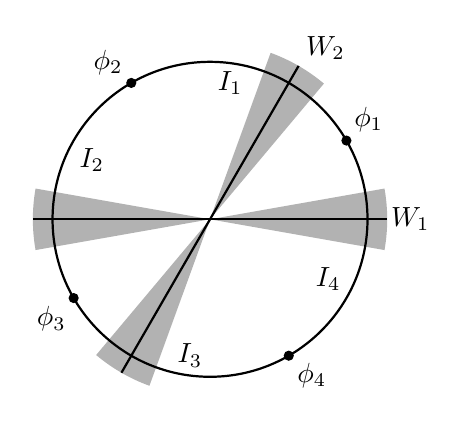
\begin{tikzpicture}
  \foreach \angle in {0, 60, 180, 240} {
    \draw[draw=none, fill=black!30] (0,0) -- (\angle-10:2.25) arc(\angle-10:\angle+10:2.25) -- cycle;
  }

  \draw[thick] (0, 0) circle (2cm);
  \foreach \angle/\label in {30/\phi_1, 120/\phi_2, 210/\phi_3, 300/\phi_4} {
    \node at (\angle:2) [circle, fill,inner sep=1.3pt,label={[label distance=-.1cm]\angle:$\label$}] {};
  }

  \draw[thick] (-2.25,0) -- (2.25,0); 
  \draw[thick] ({-2.25*cos(60)}, {-2.25 * sin(60)}) -- ({2.25*cos(60)}, {2.25 * sin(60)});
  \node at (2.25,0) [label={[label distance=-.2cm ]0:$W_1$}] {}; 
  \node at ({2.25*cos(60)}, {2.25 * sin(60)}) [label={[label distance=-.2cm]60:$W_2$}] {}; 

  \foreach \angle/\label in {75/I_1, 150/I_2, 255/I_3, 330/I_4} {
    \coordinate (p) at ({2*cos(\angle)},{2*sin(\angle)});
    \node at (p) [label={[label distance=-.2cm]{\angle+180}:$\label$}] {};
  }  
\end{tikzpicture}
  \end{center}
  \caption{\label{fig:cones}The intersection of $W_1$ and $W_2$ with the horizontal circle $S^1$. The shaded neighborhoods of $W_1$ and $W_2$ represent $\Cone_{W_1,L}$ and $\Cone_{W_2,L}$.  
  }
  \end{figure}
  
  For $\theta\in S^1$ and $t>0$, we have $d(\0,\theta^t) = t$ and $d(\theta^t, W_i) = t \sin \angle(\theta,W_i) = t |\cos\angle(\theta,U_i)|$, so 
  \begin{equation}\label{eq:plane-dist}
    d(\theta^t, W_i) - L d(\0,\theta^t) = t (\sin(\angle(\theta,W_i)) - L).
  \end{equation}
  For $p\in \HH$, let $D(p) = d(p, W_i) - L d(\0,p)$. Then $D$ is a $(1+L)$--Lipschitz function and $\Cone_{W_i,L} = D^{-1}((-\infty,0]))$; it follows that $\theta^t \in \Cone_{W_i,L}$ if and only if $\angle(\theta,W_i) \le \sin^{-1}(L)$ and that if $\sin(\angle(\theta,W_i))> L$, then 
  \begin{equation}\label{eq:cone-dist}
    d(\theta^t, \Cone_{W_i,L}) \ge \frac{t}{1+L}(\sin(\angle(\theta,W_i)) - L).
  \end{equation}
  
  By our choice of $L$, if $\angle(\theta,W_i) \ge \frac{1}{4}\angle(W_1,W_2)$, then $\theta^t \in \HH\setminus \Cone_{W_i,L}$, and whether $\theta^t\in \Cone_{V_i,L}^+$ or $\Cone_{V_i,L}^-$ depends on the sign of $\cos \angle(\theta, U_i)$.  
  
  The planes $W_1$ and $W_2$ divide $S_1$ into four arcs. Let $\phi_1, \phi_2, \phi_3, \phi_4 \in S^1$ be the midpoints of the four arcs in counterclockwise order, and let $I_j$ be the closed arc from $\phi_j$ to $\phi_{j+1}$ (taking $\phi_5=\phi_1$). Then $\angle(\phi_j,W_i) \ge \frac{1}{2}\angle(W_1,W_2)$ for all $i$ and $j$, so $\phi_j \in \Cone_{V_1,L}^\pm \cap \Cone_{V_2,L}^\pm$ for some choice of signs. After possibly swapping $\Cone_{V_i,L}^+$ and $\Cone_{V_i,L}^-$ and choosing the order of the $\phi_j$'s, we may suppose that $I_1\subset \Cone_{V_1,L}^+$, $I_2\subset \Cone_{V_2,L}^+$, $I_3\subset \Cone_{V_1,L}^-$, and $I_4\subset \Cone_{V_2,L}^-$, as in Figure~\ref{fig:cones}.

  Let $F=(f_1,f_2)\from \HH\to \R^2$, where the $f_i$'s are the signed distance functions
  $$f_i(v) = \begin{cases}
    d(v,\Gamma_i) & v \in \Gamma_i^+ \\
    0 & v \in \Gamma_i \\
    -d(v,\Gamma_i) & v \in \Gamma_i^-.
  \end{cases}$$
  We claim that if $t>0$ is sufficiently large, and $\gamma_t\from S^1\to \HH$, $\gamma_t(\theta)=\theta^t$, then the composition $F\circ \gamma_t$ has winding number $1$ around the origin.

  By \eqref{eq:cone-dist}, if $|\cos \angle(\theta, U_i)| > L$, then 
  $$d(\theta^t, \Cone_{W_i,L}) \ge \frac{t}{1+L} (|\cos \angle(\theta,U_i)| - L)  
  \ge \frac{t}{2} (|\cos \angle(\theta,U_i)| - L).$$
  Thus, if $g\in \Gamma_i$, $\theta\in S^1$, and $t>0$, then 
  \begin{equation}\label{eq:signed-on-graph}
    |f_i(g\theta^t)| \ge d(g\theta^t, g\Cone_{W_i,L}) \ge \frac{t}{2} (|\cos \angle(\theta,U_i)| - L),
  \end{equation}
  and the sign of $f_i(g\theta^t)$ agrees with the sign of $\cos \angle(\theta,U_i)$. 
  
  For any $h\in \HH$, we have
  $$g h g^{-1} h^{-1} = [g,h] = Z^{\omega(\pi(g),\pi(h))}$$
  and $|\omega(\pi(g),\pi(h))|\le \|g\|_K \|h\|_K$. In particular,
  $$d(h, g h g^{-1}) \le 2 \sqrt{\|g\|_K \|h\|_K}.$$
  Therefore,
  $$d(g \theta^{t}, \theta^t) = \|\theta^{-t} g^{-1} \theta^{t}\|_K  = \|[\theta^{-t},g^{-1}] \cdot g^{-1}\|_K \le 2\sqrt{|t|\|g\|_K} + d(\0, g) = O(\sqrt{t})$$
  as $t\to \infty$ with constant depending on $\|g\|_K$. If $|\cos \angle(\theta,U_i)|>L$, then the fact that $f_i$ is $1$--Lipschitz implies
  \begin{equation}\label{eq:signed-off-graph}
    |f_i(\theta^t)| \ge |f_i(g\theta^t)| - d(g\theta^t, \theta^t) \ge \frac{t}{2} (|\cos \angle(\theta,U_i)| - L) - O(\sqrt{t}),
  \end{equation}
  which is positive when $t$ is sufficiently large.

  A compactness argument combined with \eqref{eq:signed-off-graph} implies that if $t$ is sufficiently large, then
  $f_1(\gamma_t(I_1))>0$, $f_2(\gamma_t(I_2))>0$, $f_1(\gamma_t(I_3))<0$, and $f_2(\gamma_t(I_4))<0$. Therefore, $F(\gamma_t(S_1))\subset \R^2\setminus \0$ and $F\circ \gamma_t$ has winding number $1$ around $\0$. It follows that if $\Sigma$ is a surface in $\HH$ with boundary $\gamma_t$, then there is some $p\in \Sigma$ such that $F(p)=\0$ and thus $p\in \Gamma_1\cap \Gamma_2$. Thus $E=\Gamma_1\cap \Gamma_2$ is nonempty.

  Now, we claim that $E$ is connected and has no endpoints. Suppose that $\0\in E$. Then for any $\delta>0$, \eqref{eq:signed-on-graph} implies that $f_1(\gamma_\delta(I_1))>0$, $f_2(\gamma_\delta(I_2))>0$, $f_1(\gamma_\delta(I_3))<0$, and $f_2(\gamma_\delta(I_4))<0$, so any surface with boundary $\gamma_\delta$ contains an element of $E$. In particular, $\gamma_\delta$ divides the boundary $\partial B(\0,\delta)$ into two halves  $\Sigma^+=\{v\in \partial B(\0,\delta) : v\succ \0\}$ and $\Sigma^-=\{v\in \partial B(\0,\delta) : v\prec \0\}$, and each half contains an element of $E$. That is, there are points $q^\pm \in E$ such that $d(\0,q^\pm)=\delta$ and $q^-\prec \0 \prec q^+$. (Since $\lambda \ge \frac{1}{4}$, by Lemma \ref{lem:Properties}.(\ref{Item3}), $E$ is totally ordered.) By left-invariance, for any $p\in E$, there are $q^\pm \in E$ such that $d(p,q^\pm)=\delta$ and $q^-\prec p \prec q^+$.

  This property lets us describe the structure of $E$. By Lemma~\ref{lem:topologies}, the order on $E$ is complete and separable. We claim that it is dense. Suppose that $v, w\in E$ and $v\prec w$. Then $z(v^{-1}w)>0$. By Lemma~\ref{lem:Properties}.(\ref{Item4}), there is a $c_\lambda>0$ such that if $v\prec w \prec q$, then $z(v^{-1}q)\ge c_\lambda z(v^{-1}w)$ and thus
  $$d(v,q) \ge 2\sqrt{c_\lambda z(v^{-1}w)}.$$
  Let $\delta = \sqrt{c_\lambda z(v^{-1}w)}$. By the above, there is a $q\in E$ such that $v\prec q$ and $d(v,q)=\delta$. By our choice of $\delta$, we have $v\prec q \prec w$. Thus the order on $E$ is complete, separable, and dense. As in the proof of Proposition~\ref{prop:intervals}, $E$ is order-isomorphic to $(0,1)$ and thus it is homeomorphic to $(0,1)$, i.e., it is connected and does not contain any endpoints.
\end{proof}

\begin{proof}[Proof of Theorem \ref{thm:intersections}]
    Let $L'\in (0,1)$ be small enough such that Lemma~\ref{lem-connectedness} holds, i.e., the intersection of any $L'$--iLip graph over $W_1$ and any $L'$--iLip graph over $W_2$ is a nonempty connected vertical curve without endpoints. We may suppose that $L'$ is small enough that $\Cone_{W_1,L'}\cap\Cone_{W_2,L'}$ contains no horizontal vectors.

    By Lemma \ref{lem:containment}, there is a $\lambda_0>0$ such that any $\lambda_0$--vertical curve is contained in an entire $L'$--iLip graph over any two-dimensional vertical subgroup. We claim that the theorem holds for any $\lambda > \lambda_0$.

    Let $\lambda > \lambda_0$. 
    By compactness, there is some $L = L(\lambda)\in (0,L')$ such that 
\begin{equation}\label{ContainmentCones2}
\Cone_{W_1,L}\cap\Cone_{W_2,L}\subset  \VCone_\lambda.
    \end{equation}
    We claim that $L$ satisfies part (1) of the theorem. Let $\Gamma_1$ and $\Gamma_2$ be entire $L(\lambda)$-iLip graphs over $W_1$ and $W_2$ respectively. Since $L<L'$, by Lemma~\ref{lem-connectedness}, $E=\Gamma_1\cap \Gamma_2$ is a nonempty connected vertical curve with no endpoints. 
    By \eqref{ContainmentCones2}, $E$ is $\lambda$--vertical.

    Now, we claim that $L'$ satisfies part (2) of the theorem. Let $E$ be a $\lambda$--vertical curve. By Lemma \ref{lem:containment} we can find two entire $L'$--iLip graphs $\Gamma_1$ and $\Gamma_2$ over $W_1$ and $W_2$ such that $E\subset \Gamma_1\cap\Gamma_2$. Moreover, by Lemma~\ref{lem-connectedness}, $\Gamma_1\cap\Gamma_2$ is a connected vertical curve without endpoints. 
    
    If furthermore $E$ is closed, connected, nonempty, and has no endpoints, then $E$ is both closed and open in $\Gamma_1\cap \Gamma_2$. Since $\Gamma_1\cap \Gamma_2$ is connected, this implies $E=\Gamma_1\cap \Gamma_2$ as desired.
\end{proof}

\section{Vertical curves with fractional Hausdorff dimension}\label{Proof2.5}
In this section, we construct vertical curves with fractional Hausdorff dimension and prove Theorem~\ref{thm:HausDim2}.

We start by defining some basic concepts for smooth vertical curves, including the speed and the $\mathfrak{h}$--slope.
For a smooth curve $\alpha\from I\to \HH$, we let $\alpha'\from I \to \mathfrak{h}$ denote the velocity vector of $\alpha$, left-translated to the origin, i.e.,
\begin{equation}\label{eq:left-deriv}
  \alpha'(\tau) = \frac{\mathrm{d}}{\mathrm{d}t}[\alpha(\tau)^{-1}\alpha(t)]_{t=\tau}.
\end{equation}
This lets us write $\cH^2(\alpha)$ as an integral in terms of $\alpha'$, see, e.g., \cite[page 83]{Kozhevnikov}.

\begin{lemma}\label{lem:measure-calculation}
  $\cH^2(\alpha) = \int_0^1 |z(\alpha'(t))|\ud t$.
\end{lemma}
Consequently, if $\alpha$ is a smooth curve with $|z(\alpha'(t))|=1$ for all $t$, we say that it has \emph{unit speed}. A $\lambda$--vertical curve may have $|z(\alpha'(t))|=0$ at some points, so not every $\lambda$--vertical curve has a unit-speed parameterization.

If $\gamma$ is a smooth curve and $z(\gamma'(t)) > 0$ for all $t$, we say that $\gamma$ is \emph{positively oriented}. Any such curve can be reparameterized with unit speed. If $\gamma$ is positively oriented, we define its \emph{$\mathfrak{h}$--slope} at $t$ as $\frac{z(\gamma'(t))}{|\pi(\gamma'(t))|}$ when $\pi(\gamma'(t))\ne 0$ and as $+\infty$ if $\pi(\gamma'(t)) = 0$. For $m\ge 0$, we say that $\gamma$ has $\mathfrak{h}$--slope at least $m$ if $\gamma$ is positively oriented and 
$z(\gamma'(t)) \ge m |\pi(\gamma'(t))|$ for all $t$. The $\mathfrak{h}$--slope is independent of the parameterization of $\gamma$, but rescaling a curve multiplies its $\mathfrak{h}$--slope by a constant factor.
\begin{lemma}\label{lem:slope-scale}
  Let $m, r > 0$ and let $\gamma$ be a curve with $\mathfrak{h}$--slope at least $m$. Then $s_r\circ \gamma$ has $\mathfrak{h}$--slope at least $rm$.
\end{lemma}
\begin{proof}
  For all $t$,
  $$z((s_r\circ \gamma)'(t)) = z(s_r(\gamma'(t))) = r^2 z(\gamma'(t))$$
  and
  $$\pi((s_r\circ \gamma)'(t)) = \pi(s_r(\gamma'(t))) = r \pi(\gamma'(t)),$$
  so 
  $$z((s_r\circ \gamma)'(t)) = r^2 z(\gamma'(t)) \ge m r^2 |\pi(\gamma'(t))| = m r |\pi((s_r\circ \gamma)'(t))|,$$
  as desired.
\end{proof}

A curve with positive slope is locally vertical, but not necessarily globally vertical.
\begin{lemma}\label{lem:slope-vertical}
  Let $m>0$ and let $\alpha\from I\to \HH$ be a curve with $\mathfrak{h}$--slope at least $m$. Let $s,t\in \R$ and let
  $$\sigma = \left|\int_{s}^{t} z(\alpha'(\tau))\ud\tau\right|.$$
  Then $|\pi(\alpha^{-1}(s)\alpha(t))| \le \frac{\sigma}{m}$ and 
  \begin{equation}\label{eq:slope-vertical-diff}
    \left|z(\alpha^{-1}(s)\alpha(t)) -\sigma\right| \le \frac{\sigma^2}{m^2}.
  \end{equation}
  Consequently, if $\sigma < m^2$, then
  \begin{enumerate}
  \item $\alpha^{-1}(s)\alpha(t) \in \VCone_\lambda$, where 
  $$\lambda = \frac{m^2}{\sigma} - 1,$$
  \item $d(\alpha(s)^{-1}\alpha(t), Z^{\sigma}) \le \frac{5\sigma}{m}$, so 
  $$d(\alpha(s),\alpha(t)) \le 4\sqrt{\sigma} + \frac{5\sigma}{m}.$$
  \end{enumerate}
\end{lemma}
Some condition on $\sigma$ is necessary, since one can construct closed curves with positive $\mathfrak{h}$--slope. For example, $\gamma(t) = (\cos t, - \sin t, -t)$
is a horizontal curve, so $\lambda(t) = \gamma(t)Z^{t} = (\cos t, -\sin t, 0)$ is a closed curve with $\mathfrak{h}$--slope $1$.

\begin{proof}[Proof of Lemma~\ref{lem:slope-vertical}]
  After reparameterizing and translating, and possibly swapping $s$ and $t$, we may suppose that $\alpha$ is a unit-speed curve, $s=0\le t$, and $\alpha(s)=\0$, so that $\sigma=t-s=t$. A direct computation shows that 
  \[
\alpha'(t)=\left(\alpha_x'(t),\alpha_y'(t),\alpha_z'(t)-\frac{1}{2}\alpha_x(t)\alpha_y'(t)+\frac{1}{2}\alpha_x'(t)\alpha_y(t)\right).
  \]
  Since $\alpha$ is parametrized with unit speed and has $\mathfrak{h}$--slope at least $m$ we have $z(\alpha'(t)) = 1$ and $|\pi(\alpha'(t))|\leq m^{-1}$. Integrating this inequality, we get the desired inequality $|\pi(\alpha(t))|\leq tm^{-1}$.
  
  By Cauchy--Schwarz,   
  \begin{equation}\label{eq:az-diff}
  \big|\alpha_z'(t)-1\big|=\frac{1}{2} \big|\alpha_x(t)\alpha_y'(t) -\alpha_x'(t)\alpha_y(t)\big| \le \frac{1}{2} |\pi(\alpha'(t))|\cdot |\pi(\alpha(t))| \le \frac{t}{2m^2}.
  \end{equation}
  Therefore, 
  \begin{equation}
    |\alpha_z(t)-t|=\left|\int_0^t \left(\alpha_z'(s)-1\right)\mathrm{d}s\right|\leq\int_0^t \frac{s}{2m^2}\ud s= \frac{t^2}{4m^2}\leq \frac{t^2}{m^2},
  \end{equation}
  which implies \eqref{eq:slope-vertical-diff}. The last two assertions of the lemma follow from direct calculation using \eqref{eq:def-koranyi} and \eqref{eqn:Vcone}.
\end{proof}


The goal of this section is to prove the following proposition, which immediately implies Theorem~\ref{thm:HausDim2}. 
\begin{prop}\label{prop:curves}
  Let $\lambda,\lambda',\epsilon > 0$, with $\lambda'<\lambda$, and let $\alpha\from [0,\ell]\to \HH$ be a unit-speed $\lambda$--vertical curve. Suppose that $\alpha$ has $\mathfrak{h}$--slope at least $m$ for some $m>0$. There are smooth $\lambda'$--vertical curves $\gamma_1,\gamma_2 \from [0,\ell] \to \HH$ connecting $\alpha(0)$ to $\alpha(\ell)$ such that $\cH^2(\gamma_1) < \epsilon$, $\cH^2(\gamma_2) >\epsilon^{-1}$, and $d_{\mathrm{Haus}}(\alpha,\gamma_i) < \epsilon$ for each $i$, where $d_{\mathrm{Haus}}$ denotes the Hausdorff distance. 
  
  Furthermore, there are $\lambda'$--vertical curves $\tau_1, \tau_2 \from [0,1] \to \HH$ connecting $\alpha(0)$ to $\alpha(\ell)$ such that $d_{\mathrm{Haus}}(\alpha,\tau_i) < \epsilon$, and $\dim_H(\tau_1)<2<\dim_H(\tau_2)$.
\end{prop}

The curves we will construct  look like helixes at many different scales, as in Figure~\ref{fig:Hausdim2}. The idea of this construction is that if $\beta$ is a curve with $\mathfrak{h}$--slope at least $m$ and if $\rho>0$ is large, then, by Lemma~\ref{lem:slope-scale}, the rescaling $s_{m^{-1} \rho} \circ \beta$ has $\mathfrak{h}$--slope at least $\rho$. By Lemma~\ref{lem:slope-vertical}, the intersection of $s_{m^{-1} \rho} \circ \beta$ with any unit ball is close to a vertical segment. Equivalently, the intersection of $\beta$ with any ball of radius $m\rho^{-1}$ is close to a vertical segment. 

Thus, given a starting curve $\gamma$ with $\mathfrak{h}$--slope bounded away from zero, there is some $r_1$ so that the intersection of $\gamma$ with any ball of radius $r_1$ is close to a vertical segment. We can perturb $\gamma$ by replacing these vertical segments with helixes, and this replace can increase or decrease the measure of $\gamma$. Furthermore, if the perturbations are small, the perturbed curve still has $\mathfrak{h}$--slope bounded away from zero, so we can repeat the process at a smaller scale $r_2$ and so on to construct curves with arbitrarily large or small Hausdorff measure; these curves and their limits will satisfy Proposition~\ref{prop:curves}.

We will need the following lemmas.
\begin{lemma}\label{lem:inductive-curves}
  There are $\beta, r>0$ ($\beta=\frac{1}{400}$ and $r>1000$ suffice) with the following property.
  Let $0<\kappa<1$. For any $\phi=\pm 1$, any compact interval $I$, and any smooth curve $\gamma\from I \to \HH$ with $\mathfrak{h}$--slope at least $\kappa^{-1}$ and $\mathcal{H}^2(\gamma)\geq 1$, there is a smooth curve $\tilde{\gamma}\from I\to \HH$ with the same endpoints as $\gamma$ which satisfies the following properties:
  \begin{enumerate}
  \item $\tilde{\gamma}$ has $\mathfrak{h}$--slope at least $\kappa^{-1} r^{-1}$.
  \item For all $t$, $d(\gamma(t),\tilde{\gamma}(t))\le \kappa r^{-1}$.
  \item If $\phi = 1$, then for all $t$,
    $$(1+2\beta \kappa^2) z(\gamma'(t)) \le z(\tilde{\gamma}'(t)) \le (1+6\beta \kappa^2) z(\gamma'(t)).$$
    If $\phi = -1$, then for all $t$,
    $$(1-6\beta \kappa^2) z(\gamma'(t)) \le z(\tilde{\gamma}'(t)) \le (1-2\beta \kappa^2) z(\gamma'(t)).$$
  \end{enumerate}
\end{lemma}

We defer the proof of Lemma~\ref{lem:inductive-curves} to the end of the section.

\begin{lemma}\label{lem:leeway}
  Let $0 < \lambda' < \lambda$. There is a $\delta > 0$ such that if $v\in \VCone_\lambda$ and $g,g'\in B(\0,\delta \sqrt{|z(v)|})$, then
  $g v g' \in \VCone_{\lambda'}$.
\end{lemma}
\begin{proof}
  Let $K=\{w\in \VCone_\lambda : |z(w)|=1\}$. This set is a compact subset of the interior of $\VCone_{\lambda'}$, so there is a $\delta>0$ such that 
  $$B(\0,\delta) \cdot K \cdot B(\0,\delta) \subset \VCone_{\lambda'}.$$
  We claim that this $\delta$ satisfies the lemma. Let $v\in \VCone_\lambda$. The lemma is trivial when $v=\0$, so we may suppose that $|z(v)|\ne 0$. Let $s=s_{\sqrt{|z(v)|}}$ so that $|z(s(v))|=1$. By the scale-invariance of $\VCone_\lambda$,
  $$s^{-1}(g v g')= s^{-1}(g)s^{-1}(v)s^{-1}(g') \in B(\0,\delta) \cdot K\cdot B(\0,\delta),$$
  so $s^{-1}(g v g') \in \VCone_{\lambda'}$ and thus $g v g'\in \VCone_{\lambda'}$, as desired.
\end{proof}


Given these lemmas, we can prove Proposition~\ref{prop:curves}.
\begin{proof}[Proof of Proposition~\ref{prop:curves}]
  Let $c=c_\lambda>0$ be as in Lemma~\ref{lem:Properties}.(\ref{Item4}); we can take $c<\frac{1}{4}$. 
By Lemma~\ref{lem:leeway}, there is a $\delta>0$ such that if $v\in \VCone_\lambda$ and $g,g'\in B(\0,\delta\sqrt{|z(v)|})$, then $g v g' \in \VCone_{\lambda'}$.   Let 
$$
\kappa = \min \left\{(\lambda+1)^{-2},\frac{1}{10}, \frac{\delta\sqrt{c}}{4},\frac{\epsilon}{2}\right\}
$$

  After a rescaling and reparametrization we may suppose $\alpha$ is a positively oriented unit-speed curve, that $\ell = \cH^2(\alpha) \ge 1$, and that $\alpha$ has $\mathfrak{h}$--slope at least $\kappa^{-1}$. We use Lemma~\ref{lem:inductive-curves} to construct a sequence of curves $\alpha_0,\alpha_1,\dots\from [0,\ell] \to \HH$ as follows. Let $\beta=\frac{1}{400}$ and $\rho=1000$ so that Lemma~\ref{lem:inductive-curves}. holds with $r=\rho$. Take $\phi=\pm1$.   
  Let $\alpha_0=\alpha$. 

  Suppose that we have constructed $\alpha_i$ such that $\alpha_i\from [0,\ell]\to \HH$ is a smooth curve with $\mathfrak{h}$--slope at least $m_i := \kappa^{-1} \rho^{-i}$ and $\ell_i:=\cH^2(\alpha_i)\ge 2^{-i}$. This is already satisfied for $i=0$. Let $\gamma_i(t) = s_{\rho^{i}} \circ \alpha_i$; then by Lemma~\ref{lem:slope-scale}, $\gamma_i$ has $\mathfrak{h}$--slope at least $\kappa^{-1}$ and $\cH^2(\gamma_i) \ge 1$, so we can apply Lemma~\ref{lem:inductive-curves} with $r=\rho$ to $\gamma_i$ to obtain a curve $\tilde{\gamma}_i$. Let
  $\alpha_{i+1}(t) = s_{\rho^{-i}}\circ \tilde{\gamma}_i.$

  Let $\ell_{i+1}:=\cH^{2}(\alpha_{i+1})$. Then $\ell_{i+1}\ge \frac{1}{2} \ell_i\ge 2^{-i-1}$ and, by Lemma~\ref{lem:slope-scale}, $\alpha_{i+1}$ has $\mathfrak{h}$--slope at least $\kappa^{-1}\rho^{-i-1}$, so we can repeat this process inductively to construct $\alpha_i$ for all $i$. Furthermore, using Lemma~\ref{lem:inductive-curves} for all $i$:
  \begin{enumerate}
  \item $\alpha_i$ has $\mathfrak{h}$--slope at least $\kappa^{-1}\rho^{-i}$.
  \item For all $t$, $d(\alpha_i(t),\alpha_{i+1}(t)) \le \kappa \rho^{-i-1}$. Therefore, for all $j<i$,
    \begin{equation}\label{eq:alpha-diff}
      d(\alpha_j(t),\alpha_{i}(t)) \le \sum_{n=j}^{i-1} d(\alpha_n(t),\alpha_{n+1}(t)) \le 2\kappa \rho^{-j-1}.
    \end{equation}
  \item If $\phi = 1$, then for all $t$,
    \begin{equation}\label{eq:zalpha-plus}
      (1+2\beta \kappa^2) z(\alpha_i'(t)) \le z(\alpha_{i+1}'(t)) \le (1+6\beta \kappa^2) z(\alpha_i'(t)).
    \end{equation}
    If $\phi = - 1$, then for all $t$,
    \begin{equation}\label{eq:zalpha-minus}
      (1-6\beta \kappa^2) z(\alpha_i'(t)) \le z(\alpha_{i+1}'(t)) \le (1-2\beta \kappa^2) z(\alpha_i'(t)).
    \end{equation}
  \end{enumerate}

  Next, we introduce some notation and prove some metric bounds on the $\alpha_i$ in preparation to show that each curve $\alpha_i$ is $\lambda'$--vertical. For each $i$, let 
  \begin{equation}\label{eq:sigma-j}
    \Sigma_i(t) = \int_{0}^{t} z(\alpha_i'(\tau))\ud\tau,
  \end{equation}
  so that $\Sigma_i(\ell)=\ell_i$.
  Since $\alpha_i$ has positive slope, $\Sigma_i$ is monotone increasing. 
  
  Let $0\le s \le t \le \ell$ and for each $i$, let
  $$\sigma_i=\Sigma_i(t)-\Sigma_i(s)= \int_{s}^{t} z(\alpha_i'(\tau))\ud\tau$$
  and let $v_i=\alpha_i(s)^{-1}\alpha_i(t)$.
  
  We want to bound $v_i$; we start with the case that $s$ and $t$ are close together. Suppose that $i\ge 0$ and $\sigma_i\le \rho^{-2i}$.
  Recall that $\alpha_i$ has $\mathfrak{h}$--slope at least $m_i=\kappa^{-1}\rho^{-i}$. By Lemma~\ref{lem:slope-vertical}, $v_i\in \VCone_L$, where
  $$
  L = \frac{m_i^2}{\rho^{-2i}} - 1 = \kappa^{-2} - 1 >\lambda$$
  and
  $$
  |z(v_i) - \sigma_i| \le \frac{1}{m_i^2}\sigma_i^2 \le \frac{\rho^{-2i}}{\kappa^{-2}\rho^{-2i}} \sigma_i\le \frac{1}{2} \sigma_i.
  $$
  Therefore, 
  \begin{equation}\label{eq:slope-bound}
    \frac{\sigma_i}{2}\le |z(v_i)| \le \frac{3\sigma_i}{2} \text{ and } v_i \in \VCone_\lambda \qquad \text{if $\sigma_i\le \rho^{-2i}$.}
  \end{equation}

  By choosing $j$ carefully, we can use \eqref{eq:slope-bound} to get upper and lower bounds on $v_j$. Suppose that $|s-t| \le 1$ and let $j$ be the largest integer such that $\sigma_j \le \rho^{-2j}$. By the maximality of $j$, $\sigma_{j+1} \ge \rho^{-2j-2}$.
  Regardless of $\phi$, \eqref{eq:zalpha-plus} and \eqref{eq:zalpha-minus} imply $z(\alpha_j'(\tau))\ge \frac{1}{2} z(\alpha_{j+1}'(\tau)),$
  so $\sigma_{j}\ge \frac{1}{2} \rho^{-2j-2}$. Combined with \eqref{eq:slope-bound}, this implies
  \begin{equation}\label{eq:z-upperlower}
  v_j\in \VCone_\lambda,\qquad  \frac{1}{2} \rho^{-2j-2}\le \sigma_j \le \rho^{-2j},\qquad
    \frac{\sigma_j}{2}\le z(v_j) \le\frac{3\sigma_j}{2}.
  \end{equation}

  We use \eqref{eq:z-upperlower} and Lemma~\ref{lem:leeway} to prove that the $\alpha_i$ are $\lambda'$--vertical. 

  Let $i\ge 0$, let $0\le s\le t\le \ell$, and let $v_i$ and $\sigma_i$ be as above. We claim that $v_i\in \VCone_{\lambda'}$; we consider three cases. First, if $\sigma_i \le \rho^{-2i}$, then $v_i\in \VCone_{\lambda}$ by \eqref{eq:slope-bound}. 
  
  Second, suppose that $\sigma_i > \rho^{-2i}$ but $|s-t|<1$. Let $j$ be the largest integer such that $\sigma_j \le \rho^{-2j}$; note that $j<i$. Then $v_j\in \VCone_\lambda$ by \eqref{eq:slope-bound}; we will use Lemma~\ref{lem:leeway} to show that $v_i\in \VCone_\lambda'$.
  
  By \eqref{eq:alpha-diff}, there are $g,g'\in B(\0,2\kappa\rho^{-j-1})$ such that $\alpha_i(s) = \alpha_j(s) g$ and $\alpha_i(t) = \alpha_j(t) g'$, so
  $$v_i = \alpha_i(s)^{-1} \alpha_i(t) = g^{-1} \alpha_j(s)^{-1}\alpha_j(t)g' = g^{-1}v_j g'.$$
  By \eqref{eq:z-upperlower}, $z(v_j)\ge \frac{1}{4} \rho^{-2j-2} \ge \frac{c}{2}\rho^{-2j-2}$, and by our choice of $\kappa$, 
  $$2\kappa \rho^{-j-1} \le \delta \sqrt{\frac{c}{2}}\rho^{-j-1} \le \delta \sqrt{|z(v_j)|}.$$
  Lemma~\ref{lem:leeway} then implies that $v_i\in \VCone_{\lambda'}$.
  
  Finally, suppose that $|s-t|\ge 1$. Then $v_0\in \VCone_\lambda$ by the verticality of $\alpha_0$. Since $\alpha_0$ is a unit-speed curve, we have $\sigma_0 = t - s \ge 1$, i.e., $s+1\le t$. Since $\alpha_0$ has $\mathfrak{h}$--slope at least $\kappa^{-1}$ and $\kappa^{-1}\ge 10$, Lemma~\ref{lem:slope-vertical} implies that
  $$z(\alpha_0(s)^{-1}\alpha_0(s+1)) \ge 1 - \frac{1}{100} \ge \frac{1}{2}.$$
  Since $\alpha_0$ is positively oriented, $\alpha_0(s)\preceq \alpha_0(s+1)\preceq \alpha_0(t)$, so by \eqref{eq:coarse-monotone}, $z(v_0) \ge c z(\alpha_0(s)^{-1}\alpha_0(s+1)) \geq \frac{c}{2}$. We conclude as above; by \eqref{eq:alpha-diff}, there are $g, g'\in B(\0,2\kappa\rho^{-1})$ such that $v_i = g^{-1}v_0g'$, so by Lemma~\ref{lem:leeway}, $v_i\in \VCone_{\lambda'}$. These three cases are the only possibilities, so $\alpha_i$ is $\lambda'$--vertical for all $i$.

  When $\phi=1$, we have $\ell_{i+1}\ge (1+2\beta\kappa^2) \ell_i$, so $\ell_i\to \infty$ as $i\to \infty$; when $\phi = -1$, $\ell_{i+1}\le (1-2\beta\kappa^2) \ell_i$, so $\ell_i\to 0$ as $i\to \infty$. Thus, when $\phi=1$, this construction produces a family of $\lambda'$--vertical curves with arbitrarily large lengths, and when $\phi=-1$, it produces curves with arbitrarily small lengths. Taking also into account that $\kappa\leq \epsilon/2$, and \eqref{eq:alpha-diff}, this proves the first part of the proposition.

  It remains to construct vertical curves with Hausdorff dimension greater or less than $2$. For all $t$, let $\zeta(t) = \lim_{i\to\infty} \alpha_i(t)$. This limit exists thanks to \eqref{eq:alpha-diff}. Since $\VCone_{\lambda'}$ is closed, $\zeta$ is $\lambda'$--vertical.

  Let
  $$m_\phi =
  \begin{cases}
    1-6\beta \kappa^2 & \phi = -1 \\
    1+2\beta \kappa^2 & \phi = 1,
  \end{cases}$$
  $$M_\phi =
  \begin{cases}
    1-2\beta \kappa^2 & \phi = -1 \\
    1+6\beta \kappa^2 & \phi = 1,
  \end{cases}$$
  so that we can combine \eqref{eq:zalpha-plus} and \eqref{eq:zalpha-minus} into
  \begin{equation}\label{eq:mphi}
    m_\phi z(\alpha_i'(t)) \le z(\alpha_{i+1}'(t)) \le M_\phi z(\alpha_i'(t)).
  \end{equation}

  Let
  $$c_\phi = \frac{\log \rho}{\log (\rho^2M_\phi)} = \frac{1}{2+ \log_\rho M_\phi}$$
  $$C_\phi = \frac{\log \rho}{\log (\rho^2m_\phi)} = \frac{1}{2+ \log_\rho m_\phi}.$$
  We claim that for all $s, t\in [0,\ell]$ such that $s<t$ and $|s-t|\le 1$, we have
  \begin{equation}\label{eq:zeta-holder}
    |s-t|^{C_\phi} \lesssim_\lambda d(\zeta(s),\zeta(t)) \lesssim_\lambda |s-t|^{c_\phi}.
  \end{equation}

  As above, for all $i$, let $\sigma_i =\Sigma_i(t)-\Sigma_i(s)$ and $v_i=\alpha_i(s)^{-1}\alpha_i(t)$, and let $j$ be the largest integer such that $\sigma_j \le \rho^{-2j}$. By \eqref{eq:z-upperlower},  $\frac{1}{4} \rho^{2j-2}\le z(v_j)\le \frac{3}{2}\rho^{-2j}$ and $v_j\in \VCone_\lambda$, so
  $$\frac{1}{2}\rho^{-j-1} \le \sqrt{|z(v_j)|} \le d(\alpha_j(s),\alpha_j(t)) \lesssim_\lambda \rho^{-j}.$$
  By \eqref{eq:alpha-diff}, 
$d(\zeta(\tau), \alpha_j(\tau)) \le 2\kappa \rho^{-j-1}$ for all $\tau$, so $\frac{1}{4} \rho^{-j-1}\le d(\zeta(s),\zeta(t)) \lesssim_\lambda \rho^{-j}$, i.e., $d(\zeta(s),\zeta(t)) \approx_\lambda \rho^{-j}$.

  By \eqref{eq:mphi},
  $$m_\phi^{j}|s-t|\le \sigma_j \le M_\phi^{j}|s-t|.$$
  Since $\sigma_j\approx \rho^{-2j}$,
  $$(\rho^{2}M_\phi)^{-j} \lesssim |s-t| \lesssim (\rho^{2}m_\phi)^{-j}.$$
  Therefore,
  $$|s-t|^{c_\phi} \gtrsim (\rho^{2}M_\phi)^{-jc_\phi} = \rho^{-j} \approx_\lambda d(\zeta(s),\zeta(t))$$
  and
  $$|s-t|^{C_\phi} \lesssim (\rho^{2}m_\phi)^{-jC_\phi} = \rho^{-j} \approx_\lambda d(\zeta(s),\zeta(t)),$$
  which proves \eqref{eq:zeta-holder}. Thus, $\zeta$ is a locally bi-Hölder map, and
  $$\dim_H(\zeta(I)) \in [C_\phi^{-1}, c_\phi^{-1}] = [2 + \log_\rho m_\phi, 2+ \log_\rho M_\phi].$$
  If $\phi=1$, this implies $\dim_H(\zeta(I))>2$; if $\phi=-1$, this implies $\dim_H(\zeta(I))<2$, as desired. 
\end{proof}

\begin{proof}[Proof of Lemma \ref{lem:inductive-curves}]   
    Let us fix $\beta=\frac{1}{400}$, and take $r>1000$.
    
    We first reparametrize $\gamma\from I\to\HH$ with unit speed. Let $\ell=\mathcal{H}^2(\gamma)\geq 1$. Suppose that $I=[a,b]$ and let $\sigma\from I \to \R$,
    $$\sigma(t) = \int_a^t z(\gamma'(\tau))\ud \tau.$$
    Then $\sigma'(t)>0$ for all $t$ and $\sigma(b)=\ell$, so we define $\lambda\from [0,\ell]\to \HH$, $\lambda(t) = \gamma(\sigma^{-1}(t))$. This is a smooth, unit-speed curve.
    
    We apply a perturbation with wavelength approximately $2\pi r^{-2}$ to $\lambda$.
    Let $\alpha = \big\lceil\frac{r^2 \ell}{2\pi}\big\rceil$ and $\xi=\frac{2\pi \alpha}{\ell}$. Since $r^2\ell > 1000^2$, we have $\frac{r^2 \ell}{2\pi} \le \alpha\le\frac{r^2 \ell}{\pi}$ and $r^2 \le \xi \le 2r^2$.
    
    Let $v\from [0,\ell] \to \HH$,
    $$v(t) = \frac{\kappa}{8r} (\cos(\xi t)X -\phi\sin(\xi t)Y).$$
    Let $w(s) = v(0)^{-1} v(s)$ and let
    \[
    \tilde \lambda(s):=\lambda(s)\cdot w(s).
    \]
    Then $w(0)=w(\ell)=\0$, so the endpoints of $\tilde\lambda$ and $\lambda$ coincide. 
    
    We claim that $\tilde{\lambda}$ satisfies versions of properties (1)--(3), i.e., $\tilde{\lambda}$ has $\mathfrak{h}$--slope at least $\kappa^{-1}r^{-1}$, $d(\lambda(t),\tilde{\lambda}(t))\le \kappa r^{-1}$, and $z(\tilde{\lambda}'(t))$ is between $1 + 2\phi \beta \kappa^2$ and $1 + 6 \phi\beta \kappa^2$ for all $t$.
    
    First, note that $d(\0,v(t)) = \frac{\kappa}{8}r^{-1}$ for all $t$, so $d(\lambda(t),\tilde{\lambda}(t))=d(\0,w(t))\leq \kappa r^{-1}$. 

    Next, we bound $|\pi(\tilde{\lambda}'(t))|$ and $z(\tilde{\lambda}'(t))$ in order to prove the remaining properties.
    By \eqref{eq:left-deriv},
  \begin{align*}
    \tilde{\lambda}'(\tau) & =
                      \frac{\mathrm{d}}{\mathrm{d}t} [w(\tau)^{-1}(\lambda(\tau)^{-1}\lambda(t))\cdot w(\tau) \cdot w(\tau)^{-1} w(t) ]_{t=\tau} \\
                    & = \Adj_{w(\tau)^{-1}}(\lambda'(\tau)) + w'(\tau),
  \end{align*}
  where $\Adj_{g}(v) = \frac{\mathrm{d}}{\mathrm{d}t}[g \exp(tv) g^{-1}]_{t=0}$.

  We calculate
  $$\Adj_{g}(v) = v + \omega(\pi(g),\pi(v)) Z,$$
  where $\omega$ is the area form on $\R^2$. Then $\Adj_{g}(v) - v\in \langle Z\rangle$ and
  $$
  |\Adj_{g}(v) - v| \leq |\pi(g)| |\pi(v)|,
  $$
  so
  \begin{equation}\label{eq:pi-diff}
    \pi(\tilde{\lambda}'(t)) = \pi(\lambda'(t)) + \pi(w'(t)),
  \end{equation}
  and
  \begin{align}\label{eq:z-diff}
    \left|z(\tilde{\lambda}'(t)) - \left(z(\lambda'(t)) + z(w'(t)\right)\right|& = \left|z\left(\Adj_{w(t)^{-1}}(\lambda'(t)) - \lambda'(t)\right)\right| \\
  \notag  & \le \big|\pi(w(t))\big| \big|\pi(\lambda'(t))|\big.
  \end{align}
  
  Furthermore,
  \begin{equation}
  w'(t) = v'(t) = \frac{\kappa\xi r^{-1}}{8} v'(\xi t)+\frac{\kappa^{2}r^{-2}\xi}{128}\phi Z,
  \end{equation}
  so, using that $\ell\ge \alpha\pi r^{-2}$,
  \begin{equation}\label{eq:pi-wt}
    |\pi(w'(t))| =\frac{\kappa\xi r^{-1}}{8}=\frac{2\kappa\alpha\pi r^{-1}}{8\ell} \leq \frac{2\kappa\alpha\pi r^{-1}}{8\alpha\pi r^{-2}}\leq \frac{1}{4}\kappa r.
  \end{equation}

  Since $r^2 \le \xi \le 2r^2$, we have 
  \begin{equation}\label{eq:z-wtphi}
  \frac{\kappa^2}{128}\leq |z(w'(t))| =\frac{\kappa^2 r^{-2}\xi}{128}  \leq \frac{\kappa^2}{64},
  \end{equation}
  and $z(w'(t))$ has the same sign as $\phi$. 

  This lets us bound $\tilde{\lambda}'(t)$. 
  Since $\lambda$ is unit-speed and has $\mathfrak{h}$--slope at least $\kappa^{-1}$, we have $z(\lambda'(t))=1$ and $|\pi(\lambda'(t))| \le \kappa$ for all $t$. By \eqref{eq:pi-diff} and \eqref{eq:pi-wt}, and since $r>4$,
  \begin{equation}\label{est-pi-gtild}
  |\pi(\tilde{\lambda}'(t))| \le |\pi(\lambda'(t))| + |\pi(w'(t))|\leq \kappa+\frac{1}{4}\kappa r \leq \frac{1}{2}\kappa r. 
  \end{equation}
  By \eqref{eq:z-diff} we have
  \begin{equation}\label{eqn:Est-gamma'}
  \begin{aligned}
  \left|z(\tilde{\lambda}'(t)) - 1 -z(w'(t))\right| &\le |\pi(w(t))|\cdot |\pi(\lambda'(t))| \\&\le \kappa r^{-1}\cdot \kappa= \kappa^2 r^{-1}.
  \end{aligned}
  \end{equation}
  
  Since $\beta=\frac{1}{400}$ and $r>1000$, if $\phi=-1$, then \eqref{eqn:Est-gamma'} and \eqref{eq:z-wtphi} imply
  \begin{equation*}
  1 - 6\beta \kappa^2 \le 1 - \frac{\kappa^2}{64}-\frac{\kappa^2}{r} \leq z(\tilde\lambda '(t)) \leq 1 - \frac{\kappa^2}{128} +\frac{\kappa^2}{r} \le 1 - 2\beta \kappa^2.
  \end{equation*}
  If $\phi = 1$, then 
  \begin{equation*}
  1 + 2\beta \kappa^2 \le 1 + \frac{\kappa^2}{128}-\frac{\kappa^2}{r} \leq z(\tilde\lambda '(t)) \leq 1 + \frac{\kappa^2}{64} +\frac{\kappa^2}{r} \le 1 + 6\beta \kappa^2.
  \end{equation*}
  In either case, $z(\tilde{\lambda}'(t))$ is between $1 + 2 \phi \beta \kappa^2$ and $1 + 6 \phi \beta \kappa^2$. In particular, $z(\tilde{\lambda}'(t)) \ge \frac{1}{2}$, so by \eqref{est-pi-gtild} the $\mathfrak{h}$-slope of $\tilde\lambda$ is at least $\frac{1}{2}\left(\frac{1}{2}\kappa r\right)^{-1}=\kappa^{-1}r^{1}$, as desired.

  Finally, for all $t\in I$, let $\tilde{\gamma}(t) = \tilde{\lambda}(\sigma(t))$. Since $\tilde{\gamma}$ is a reparametrization of $\tilde{\lambda}$, it has the same endpoints as $\gamma$ and satisfies properties (1)--(3).
\end{proof}


\subsection{Comparison with previous works}\label{sec:Previous} In \cite[Chapters 5 \& 6]{Kozhevnikov}, and \cite{KozhevnikovArticle}, A. Kozhevnikov studied properties of a class of vertical curves in the $(2n+1)$-dimensional Heisenberg group $\mathbb H^{2n+1}$. See also \cite{LeonardiMagnani, MagnaniStepanovTrevisan} for related results.

In \cite{Kozhevnikov}, Kozhevnikov called $\Gamma\subset\mathbb H^{2n+1}$ a \textit{vertical curve of the form $F^{-1}(\0)$} if the following holds. There is $F:\mathbb H^{2n+1}\to\mathbb R^{2n}$ of regularity $C^1_{\mathrm{H}}$ such that $F(\0)=\0$, $\Gamma=F^{-1}(\0)$, and $\mathrm{D}_{v}F$ is surjective for all $v\in \Gamma$. Here $\mathrm{D}_v F$ denotes the Pansu differential of $F$ at $v$. Then he proved the following theorem, and gave the following definition.

\begin{thm}[Theorem 5.3.7 \cite{Kozhevnikov}]\label{corvertical}
    Let $F\in C^1_{\mathrm H}(\mathbb H^{2n+1},\mathbb R^{2n})$ be such that $F(\0) = \0$, and $\mathrm{D}_\0 F$ is surjective. Then there is a neighborhood U of 0 such that $U\cap F^{-1}(\0)$ is a simple curve.
\end{thm}
\begin{defn}
    In \cite{Kozhevnikov}, sets of the form $U\cap F^{-1}(\0)$ as in Corollary \ref{corvertical} are called \textit{vertical curves}.
\end{defn}

We stress that (compare with Remark 5.3.2 \cite{Kozhevnikov}), our notion of $\lambda$--vertical curve is \textbf{locally} weaker than the one given in \cite{Kozhevnikov}. I.e., if $E\subset \HH$ is a vertical curve according to \cite{Kozhevnikov}, then for every $p\in E$ there are $\delta,\lambda>0$ such that $B_\delta(p)\cap E$ is a $\lambda$--vertical curve according to our definition. We notice that globally the two definitions might not be related.

We further point out that Theorem \ref{corvertical} is in analogy with the more general Proposition \ref{prop:intervals}. Moreover, in the proof of Theorem \ref{corvertical} the author proves that $U\cap F^{-1}(\0)$ is a bi-H\"older curve, compare with \cite[Theorem 5.2.14 \& Theorem 5.3.5]{Kozhevnikov}, and with our Lemma \ref{lem:biHolderonCompact}. Further parametrization results related to Theorem \ref{corvertical}, and Proposition \ref{prop:intervals} are in \cite[Theorem 1.1]{LeonardiMagnani}, and \cite[Theorem 5.6]{MagnaniStepanovTrevisan}.
\smallskip

Kozhevnikov also studied properties related to the Hausdorff dimension of vertical curves. In particular he proved Theorem \ref{thm:KozHaus} below, and constructed pathological examples (Proposition \ref{PathologicalExamples} below) that inspired our Proposition \ref{prop:curves}. 

Let us remark that as a result of the proofs of \cite[Lemma 5.4.3 \& Corollary 5.4.6 \& Corollary 5.4.8]{Kozhevnikov}, or refining our Lemma \ref{lem:biHolderonCompact}, it can be inferred that $|\dim_H(E)-2|\leq o_{\lambda\to\infty}(1)$ for every $\lambda$--vertical curve $E\subset \HH$.  But, in contrast with the result proved by Kozhevnikov in the Theorem \ref{thm:KozHaus} below, an arbitrary $\lambda$--vertical curve might not have Hausdorff dimension 2, as we showed in Proposition \ref{prop:curves}.

\begin{thm}[Proposition 5.3.10 \& Corollary 5.4.8 \& Corollary 5.4.16 in \cite{Kozhevnikov}]\label{thm:KozHaus}
    The Hausdorff dimension of a vertical curve (according to \cite{Kozhevnikov}) is 2.
\end{thm}
\begin{prop}[Example 5.6.16, Example 5.6.17, Example 5.6.19 in \cite{Kozhevnikov}]\label{PathologicalExamples}
    There exist  vertical curves (according to \cite{Kozhevnikov}) $\Gamma_1,\Gamma_2$ such that $\mathcal{H}^2(\Gamma_1)=0$, and $\mathcal{H}^2(\Gamma_2)=\infty$. Moreover, there exists a $2$-Ahlfors vertical curve $\Gamma_3$ (according to \cite{Kozhevnikov}) such that: for every $a\in \Gamma_3$
    \[
    0<\liminf_{r\to 0}\frac{\mathcal{H}^2(\Gamma_3\cap B_r(a))}{2r^2}<\limsup_{r\to 0}\frac{\mathcal{H}^2(\Gamma_3\cap B_r(a))}{2r^2}=1.
    \]
\end{prop}

It is not clear to us whether the examples that Kozhevnikov constructed in Proposition \ref{PathologicalExamples} are $\lambda$--vertical curves according to our definition.
